\documentclass[35pt, a0paper, portrait]{tikzposter}
\usepackage[ngerman]{babel}
\usepackage[utf8]{inputenc}
\usepackage{graphicx}

\title{\Huge\textbf{Simulated Annealing}}
\author{\huge\textbf{Erik Teichmann}}
\date{\today}
\institute{\huge Universität Potsdam}
\tikzposterlatexaffectionproofoff
\usepackage{blindtext}
\usepackage{comment}
\renewcommand{\labelenumi}{\roman{enumi}}

\usetheme{Basic}
\colorlet{backgroundcolor}{white}


 \defineblockstyle{Default1}{
    titlewidthscale=1, bodywidthscale=1, titlecenter,
    titleoffsetx=0pt, titleoffsety=0pt, bodyoffsetx=0pt, bodyoffsety=0pt,
    bodyverticalshift=0pt, roundedcorners=30, linewidth=0.4cm,
    titleinnersep=1cm, bodyinnersep=1cm
}{
    \begin{scope}[line width=\blocklinewidth, rounded corners=\blockroundedcorners]
        \ifBlockHasTitle %
           \draw[color=blocktitlebgcolor, fill=blocktitlebgcolor] (blocktitle.south west) rectangle (blocktitle.north east);
           \draw[color=blocktitlebgcolor, fill=blockbodybgcolor, opacity=0.5] (blockbody.south west) rectangle (blockbody.north east);
        \else
           \draw[color=blocktitlebgcolor, fill=blockbodybgcolor, opacity=0.5] (blockbody.south west) rectangle (blockbody.north east);
        \fi
    \end{scope}
}
\useblockstyle{Default1}


\begin{document}
\node[above right,opacity=0.5,inner sep=0pt,outer sep=0pt] at (bottomleft) {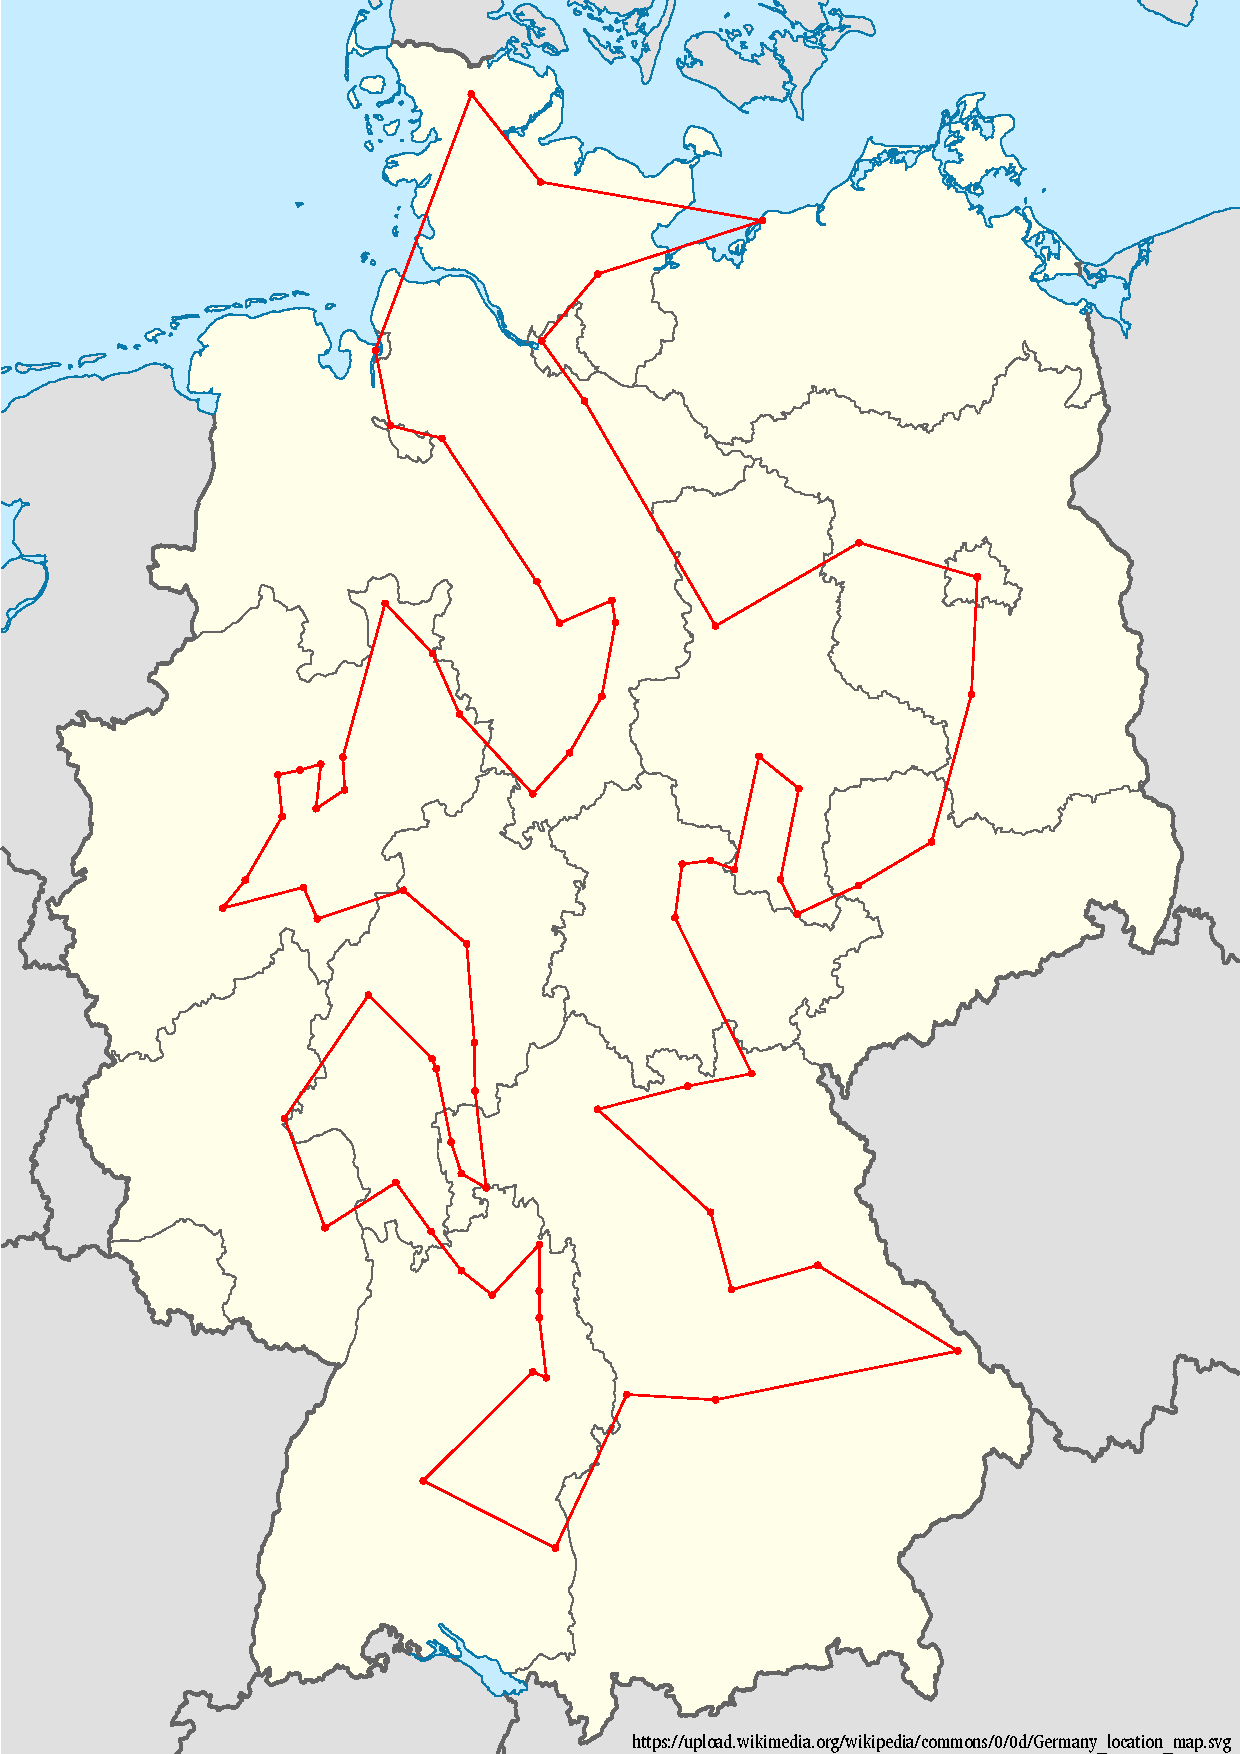
\includegraphics[width=\paperwidth,height=\paperheight]{../plt/background.pdf}};

\maketitle

\begin{columns}
  \column{0.1}
  \column{0.8}
  \block{Hintergrund}
  {
    Simulated Annealing ist ein Verfahren der Numerik. Es verwendet eine Idee der Festkörperphysik. Um möglichst reine und gleichmäßige Kristalle herzustellen wird ein Festkörper erhitzt und dann langsam abgekühlt. Durch das langsame Kühlen finden die Moleküle ihren niedrigsten energetischen Zustand besser, als durch ein schnelles Abkühlen.

    Das Simulated Annealing verwendet dasselbe Prinzip des Abkühlens, aber für Probleme der Optimierung. Die Energie ist dabei eine Kostenfunktion, also zum Beispiel eine Weglänge. Die Temperatur regelt die Änderung des Zustandes: für hohe Temperaturen ist es wahrscheinlicher, den Zustand zu wechseln, als für niedrige. Die Zustandsänderung kann dabei auch zu einer Erhöhung der Energie führen, wobei solche Änderungen für niedrige Temperaturen immer unwahrscheinlicher werden. So kann aus lokalen Minima der Energie entkommen werden, um das globale Minimum zu finden.
    }
  \column{0.1}
\end{columns}

\begin{columns}
  \column{0.4}
  \block{Problemstellung}
  {
    Das ``Traveling-Salesman'' Problem soll mithilfe von Simulated Annealing gelöst werden. Es beschreibt die geschlossene Wegstrecke durch mehrere Städte, wobei keine Stadt mehrmals besucht werden darf. Die brute-force Lösung skaliert wie $N!$ und ist somit ungeeignet für eine große Anzahl von Städten.

    Der kürzeste Weg durch 76 deutsche Städte soll gefunden werden und die Unterschiede zwischen zwei Zustandsänderungen sollen charakterisiert werden. Die Zustandsänderungen sind Flips in der Reihenfolge der Städte:

    \begin{enumerate}
      \item Die Reihenfolge von zwei zufälligen Städten wird vertauscht
      \item Die Reihenfolge zwischen zwei zufälligen Städten wird vertauscht
    \end{enumerate}

    Nach einem Flip verändert sich die Länge $L$ des Gesamtweges. Ist die neue Länge kürzer wird sie immer angenommen, ist sie aber länger wird sie nur mit der Wahrscheinlichkeit
    \begin{equation}
      p = e^{- (L_{neu} - L_{alt})/T}
    \end{equation}
    angenommen, wobei $T$ die Temperatur ist. Das erinnert an die Boltzmann-Verteilung.
  }

  \column{0.05}
  \column{0.5}
  \block{Simulation}
  {
    Die numerische Simulation wird in einem C++-Programm durchgeführt. Zuerst müssen die Längen- und Breitengrade der Städte mittels der Haversine-Formel in Distanzen zwischen den Städten umgerechnet werden. Aus der Reihenfolge der Städte kann die Wegstrecke mittels der Distanzen direkt berechnet werden.

    Um das Abkühlen zu simulieren wird die Temperatur nach einer gegeben Anzahl von Flips mit einem Cooling-Parameter $C$ multipliziert. Je näher er an 1 liegt, desto langsamer wird der Körper abgekühlt.  Die Anzahl der Flips ist zu $100N$ oder $10N$ erfolgreiche gewählt, je nachdem, was zuerst eintritt. Die Temperatur startet bei $10000$. Damit ist sie deutlich größer als eine typische Längenänderung, was die Qualität der Ergebnisse verbessert. Für jeden Cooling-Parameter werden $100$ Simulationen durchgeführt, um die Statistik der Flips beschreiben zu können.
    }
    \column{0.05}
\end{columns}

\begin{columns}
  \column{0.5}
  \block[titleoffsety=-9cm, bodyoffsety=-9cm]{Simulationsdauer}
  {
    \begin{minipage}{0.6\linewidth}
      \begin{tikzfigure}[Simulationsdauer für die verschiedenen Flip-Typen\label{fig:time}]
        \includegraphics[width=\textwidth]{../plt/time.pdf}
      \end{tikzfigure}
    \end{minipage}%
    \begin{minipage}{0.4\linewidth}
      Für die Simulationsdauern zeigt sich, dass die Simulation für Flips vom Typ 1 generell schneller ist, als für Typ 2 Flips. Vor allem für große Cooling-Parameter ist der Unterschied signifikant.

      Bei Flips vom Typ 2 wird die Reihenfolge, also die Weglänge drastisch geändert. Der Zustand nach dem Flip ist weniger abhängig von dem Zustand davor, als für die Typ 1 Flips. Damit wird ein größerer Bereich der Konfiguration getestet, aber die Annäherung an ein Minimum ist unwahrscheinlicher, deswegen werden weniger Flips akzeptiert und die Simulation läuft über eine längere Zeit.
    \end{minipage}
  }
  \column{0.5}
  \block{Qualität der verschiedenen Flips}
  {
  \begin{minipage}{0.6\linewidth}
    \begin{tikzfigure}[Verteilung der gefunden Wegstrecken für Flips vom Typ 1\label{fig:dist_1}]
      \includegraphics[width=\textwidth]{../plt/distribution_1.pdf}
    \end{tikzfigure}
    \begin{tikzfigure}[Verteilung der gefunden Wegstrecken für Flips vom Typ 2\label{fig:dist_2}]
      \includegraphics[width=\textwidth]{../plt/distribution_2.pdf}
    \end{tikzfigure}
    \end{minipage}%
    \begin{minipage}{0.4\linewidth}
      Die Ergebnisse der beiden Flips unterscheiden sich deutlich. Flips vom Typ 1 geben im allgemeinen einen größeren Mittelwert und eine größere Standardabweichung, als Flips vom Typ 2. Die gefundenen Strecken sind also meistens länger, als für die Flips vom Typ 2. Allerdings wird der Unterschied zwischen den Flips mit steigendem Cooling-Parameter immer kleiner.

      Wird auch die Simulationsdauer aus Abbildung~\ref{fig:time} in Betracht gezogen, ist es günstiger für kleine Cooling-Parameter Flips vom Typ 2 zu wählen und für große Cooling-Parameter Flips vom Typ 1.

      Die kürzeste Strecke, die gefunden wurde, beträgt $4294,14\,$km und kam aus der Simulation mit Flip-Typ 2. Sie ist im Hintergrund dargestellt.
    \end{minipage}%
  }
\end{columns}

\begin{columns}
  \column{0.5}
  \block{Literatur}
  {
    Press, W.; Numerical Recipes 3rd Edition: The Art of Scientific Computing; Cambridge University Press; 2007
  }
  \column{0.5}
\end{columns}

\end{document}
